%--------------------------------------------------------------------------------------
% Este arquivo contém a sua funtamentação teórica
%--------------------------------------------------------------------------------------
\chapter{Fundamentação Teórica}\label{sec:fundamentation}

\section{Trabalhos Relacionados}\label{trabalhosRelacionados}

Diversos trabalhos foram redigidos utilizando aprendizado por reforço no domínio da \textit{RoboCup
Soccer Simulation 2D}. Cada um desses trabalhos apresentam modelagens diferentes para o mundo.

Segundo \citeonline{sutton2018reinforcement}, a modelagem de mundo é a forma como o ambiente é representado, ou simulado. Um agente inteligente
precisa constantemente entender como está o ambiente no qual ele está inserido, por isso é
importante a definição da representação do mundo de forma que melhor se adéque ao processo de
aprendizado do agente.

Um agente empregado no aprendizado do jogo-da-velha, pode ser utilizado como exemplo. O agente
precisa entender como o jogo está sendo encaminhado para que o mesmo possa decidir em que posição
jogar, porém, o agente isolado não tem acesso ao estado do jogo e precisa de uma representação do
mesmo para que possa entendê-lo. Uma abordagem válida é numerar o tabuleiro conforme a Figura
\ref{img:ticTacToeNumbers} e atrelar a cada célula um valor que varia de acordo com o que é marcado
na mesma, uma escolha razoável é atribuir o valor ``$-1$'' à células preenchidas pelo jogador
adversário, ``$0$'' à células não preenchidas e ``$1$'' às preenchidas pelo próprio agente. Nota-se que com
essa representação o agente consegue perceber em que situação se encontra e assim escolher uma ação.
Podemos chamar cada uma das células de variável, já que nelas se encontram os valores que determinam
qual o estado atual do ambiente.

\imagem{0.6}{ticTacToeNumbers}{Representação do tabuleiro de jogo-da-velha.}{O Autor}

É fácil encontrar exemplos de problemas inseridos em ambientes que são mais complexos que o citado.
Para esses problemas é comum encontrar variáveis de valores contínuos, nesses casos é necessário
pensar em como representar as variáveis de forma discreta para que seja possível se obter um número
finito de estados. Alguns dos trabalhos citados adiante demonstram maneiras de interpretar os dados
do ambiente, para que possa ser aplicada técnica de aprendizado. 

\citeonline{gabel2008case} desenvolveram jogadores de defesa com comportamento agressivo, ou seja,
jogadores que interferem e tentam tomar a bola do jogador adversário, utilizando aprendizado por
reforço. O algoritmo desenvolvido foi chamado de NeuroHassle e utiliza redes neurais e uma abstração
do mundo em 9 dimensões, distância entre o jogador e oponente com posse de bola; vetor de velocidade
do jogador; velocidade absoluta do oponente com posse de bola; vetor de posicionamento da bola;
ângulo do corpo do jogador em relação ao oponente com posse de bola; ângulo do corpo do adversário
em relação ao gol aliado; ângulo definido pela posição do gol aliado, a posição do oponente com
posse de bola e a posição do jogador. O treinamento foi feito de forma episódica em partidas de
competições anteriores. O time gerado obteve uma taxa de falha menor que 20\% e, em competição,
cerca de 30 tomadas de bola por partida.

Uma variação de redes neurais com a utilização de \textit{backpropagation}, chamada de
\textit{Backpropagation} Resiliente (RPROP, do inglês \textit{Resilient Backpropagation}), foi
utilizada por \citeonline{Riedmiller2005Brainstormers2D} no treinamento de jogadores sem posse de
bola, ao mesmo tempo que a escolha de ações do jogador com posse de bola. Para isto, foi feita a
discretização do domínio em um Processo de Decisão Markoviano (MDP, do inglês \textit{Markovian
Decision Process}), que destacou as variáveis posição e velocidade da bola e a posição de todos os
atacantes aliados e defensores adversários, além das possíveis ações, que para os jogadores com
posse de bola consistem em passar a bola diretamente para um aliado, lançar a bola de forma que um
aliado possa interceptar a bola antes de um adversário e driblar. Já para os jogadores sem posse de
bola, é possível se mover em 8 direções a partir do local atual ou a partir do local inicial ou
mover-se para o local inicial. Este trabalho resultou no time vencedor do ano de 2007 da liga de
simulação 2D da \textit{RoboCup Soccer}.

A técnica \textit{Q-Learning} é aplicada em alguns trabalhos, como o de
\citeonline{neri2012proposal}, que utiliza desta técnica a fim de obter um sistema de tomada de
decisões focado no ataque. Nesse trabalho, as variáveis foram discretizadas em 7 estados,
caracterizados como quando é possível lançar a bola para um aliado melhor posicionado; um adversário
mais próximo está atrás do jogador com posse de bola; o adversário mais próximo está a mais de 7
metros; o adversário mais próximo está a uma distância entre 7 e 6 metros; o adversário mais próximo
está a uma distância entre 6 e 5 metros; o adversário mais próximo está a uma distância menor de 4
metros e há uma linha direta entre o jogador com posse de bola e o gol adversário. Além disso, 7
ações podem ser tomadas, são elas: passar a bola para um jogador mais próximo do gol adversário,
avançar devagar, avançar rapidamente, passar a bola para um jogador próximo, driblar, segurar a bola
ou chutar ao gol.

O modelo foi treinado e testado através da execução de conjuntos de 10 partidas. O conjunto de
treinamento se  deu contra o time base do Helios apenas na situação de posse de bola. Após o
treinamento, o time foi tuilizado no primeiro conjunto de testes contra o time base do Helios, além
disso, outro foi executado entre Helios e o PetSoccer, além de um entre o time treinado e o PetSoccer
para comparação, e por fim outro contra o time chinês WrightEagles. No primeiro conjunto foram
realizados 6 gols contra o Helios, o Helios executou 47 gols contra o PetSoccer, o time treinado
conseguiu 61  gols contra o PetSoccer e 6 contra o WrightEagles. Mostrando que a utilização do
\textit{Q-Learning} resultou numa melhoria, ganhando a maioria dos jogos. A mesma técnica foi
utilizada no time brasileiro GPR-2D de 2012, descrito em \citeonline{neriteam}, com o objetivo de
treinar a tomada de decisão para quando o jogador estiver com posse de bola. O time foi classificado
e chegou a segunda fase do campeonato mundial da \textit{RoboCup Soccer Simulation 2D}.

\citeauthoronline{liu2008regional} (\citeyear{liu2008regional} e \citeyear{liu2009sparse}), utilizam
\textit{Q-Learning} com uma abstração do conjunto de agentes como um grande agente e o conjunto de
suas ações como uma ação deste grande agente chamando os dois algoritmos criados de \textit{Regional
Cooperative Q-Learning} e \textit{Sparse Cooperative Q-Learning} (\textit{Q-Learning} Cooperativo
Regional e \textit{Q-Learning} Cooperativo Esparso). Nesses trabalhos, foram identificados estados
onde não é necessário que as ações sejam decididas em conjunto (não coordenados) e onde é
(coordenados), utilizando uma abordagem baseado em campos potenciais. Na abordagem regional foram
encontrados 5012 estados coordenados e 34390 não coordenados, já na abordagem esparsa, foram 4720
coordenados e 34682 não coordenados. O modelo foi treinado  com uma simplificação de partidas com
dois agentes defendendo e um adversário atacando e a região (reduzida para 40 x 20) dividida em 200
células. Foram rodados experimentos com 200000 e 500000 episódios comparando a técnica aplicada com
a técnica MDP e a linear independente. Para 200000 episódios foi obtida uma média de tempo de
captura de 6,57 segundos para a abordagem regional e 6,49 para a esparsa, mostrando-se o melhor
dentre 3 métodos enquanto com 500000 episódios apresenta uma média de 6,49 segundos na abordagem
regional e 6,40 na abordagem esparsa, maior apenas que o do método MDP que apresentou 6,23 segundos.

Alguns trabalhos utilizam variações do \textit{Q-Learning}, como o de 
\citeonline{carvalho2011reinforcement}, que desenvolveu um módulo de drible unindo Computador
Aritmético de Modelo Cerebelar (CMAC, do inglês \textit{Cerebellar Model Arithmetic Computer}) e
Estado-Ação-Recompensa-Estado-Ação (SARSA, do inglês \textit{State-Action-Reward-State-Action}),
este último algoritmo foi concebido como \textit{Q-Learning} conexionista modificado. Neste trabalho
a tarefa de drible foi mapeada como um problema episódico adequado para o trabalho com aprendizado
por reforço onde foram destacadas duas ações primitivas, segurar a bola e driblar (que consiste em
girar o corpo a uma determinada angulação, chutar a bola a uma distância determinada e correr para
interceptá-la) e as seguintes variáveis para compor um estado para o jogador que deverá driblar: o
ângulo global de um objeto, o ângulo relativo entre dois objetos, a distância entre dois objetos, a
altura e largura do campo e se o jogador está perto do topo ou da parte mais baixa do campo. O
treinamento do modelo criado foi feito em 5 experimentos de 50000 episódios nos quais o jogadores
não podiam recuperar a \textit{stamina} (uma forma de representar a energia do jogador) por si só utilizando o ambiente padrão e um ambiente de
treino de 20 x 20. Para testar foram executados 10000 cenários com configurações aleatórias. No fim
do treinamento foi obtido um número de vitórias de cerca de 53\% e 58\% dos testes pós-treino.

O SARSA também foi empregado em \citeonline{homem2017improving} em conjunto com o Raciocínio
Espacial Qualitativo (QSR, do inglês \textit{Qualitative Spatial Reasoning}), chamando o resultado
de Aprendizado por Reforço Qualitativo (QRL, do inglês \textit{Qualitative Reinforcement Learning})
e aplicou no desenvolvimento de um mecanismo de ataque para um time de simulação 2D. Para alcançar o
objetivo, foi utilizado o formalismo eOPRAm para discretizar o mundo em regiões qualitativas pelo
qual foram identificadas um total de 14 variáveis, são elas: a posição e orientação do jogador, a
distância e ângulo do jogador em relação à bola, se o jogador pode ou não chutar, distância e ângulo
do jogador em relação ao gol adversário, maior ângulo aberto para o gol, distância entre os aliados
e o adversário mais próximo, maior ângulo aberto para passe para cada aliado, numeração de cada
aliado e de cada adversário.

As possíveis ações foram definidas como driblar, chutar e passar a bola para um aliado específico. O
treinamento foi realizado utilizando a ferramenta Ofensa de Meio Campo (HFO, do inglês
\textit{Half-Field Offense}) 30 vezes de forma independente com 1000 episódios em 3 situações
diferentes, a primeira com apenas um jogador atacando sem nenhuma defesa, a segunda com apenas o
atacante e o goleiro e a terceira com o atacante, o goleiro e um zagueiro. Foi realizada uma
comparação da técnica utilizada com a abordagem quantitativa utilizando análise de variância. Na
primeira situação, o resultado foi de uma média de 99,3\% de gols se mostrando melhor que a
quantitativa com certeza de 95\%, enquanto a segunda e terceira situação se mostraram melhor com
margem de 1\% com 81,2\% e 47,6\% contra 78,3\% e 40,6\% respectivamente.

Além dessas variações, algumas foram empregadas com o intuito de acelerar o aprendizado, este foi o
caso de \citeonline{celiberto2007heuristic} e \citeonline{bianchi2010case}. O primeiro, utilizou a chamada \textit{Q-Learning} Acelerado Heuristicamente (HAQL, do inglês
\textit{Heuristically Accelerated Q-Learning}) para treinar um goleiro e jogador de defesa. Para
tanto, foi identificada uma heurística aplicável ao domínio e implementada no algoritmo
\textit{Q-Learning} ao mesmo tempo que é feita a discretização do mundo. As variáveis de estado para
o algoritmo foram a posição dos agentes e da bola numa grade e a direção para a qual o agente está
virado definida por norte, sul, leste ou oeste. As ações que podem ser tomadas são: mudar a direção
para a qual o agente está virado para um objeto específico, mover em direção a bola, mover-se com a
bola, passar a bola para o goleiro, chutar a bola para longe do gol mover-se para perto de um
oponente. Foram executadas 10 sessões de treinamento para o algoritmo criado, \textit{Q-Learning}
puro e a função heurística pura com 100 episódios cada, onde cada episódio consiste de uma partida
de 3000 ciclos. Foi analisada a curva de aprendizado e o número de gols sofridos para cada
algoritmo, e utilizado o teste \textit{t-student} que validou a hipótese de que a aplicação de
heurística no \textit{Q-Learning} acelera o aprendizado com nível de confiança de 95\% e uma taxa de
gols sofridos menor que as demais opções testadas.

Já \citeonline{bianchi2010case}, utilizam heurística baseada em casos para acelerar o
\textit{Minmax-Q}, que também é uma variação do \textit{Q-Learning}, para melhorar a tomada de
decisões. Os casos destacados para utilização no algoritmo foram: o caso no qual o jogador esteja com a
bola e não exista adversário no caminho, então avança para o gol; se houver um adversário bloqueando, mova
para cima ou para baixo; se houver um aliado mais próximo do gol, passa a bola e se o adversário
estiver com a bola e o jogador estiver próximo, fica na frente do adversário. O treinamento foi
feito com 20000 jogos de 10 tentativas em um domínio chamado ``futebol expandido de Littman''.
Chegou-se ao resultado de que a solução encontrada não é ótima, mas a hipótese de que o aprendizado
é acelerado foi comprovado, através do teste de \textit{t-student} e uma comparação dos resultados
das partidas e das curvas de aprendizado.

Diante dos exemplos apresentados e considerando a natureza do problema, fica decidido utilizar uma
técnica de aprendizado por reforço, mais especificamente \textit{Q-Learning}, para o treinamento de
um modelo de tomada de decisões de defesa do time em desenvolvimento, \textit{FutVasf2D}.

\section{Aprendizado por Reforço}\label{aprendizado}

Segundo \citeonline{shalev2014understanding}, aprendizado por reforço é uma técnica de aprendizado
intermediária, entre supervisionado e não supervisionado, onde o agente precisa realizar mais
previsões durante os ``testes''.

\citeonline{russell2016artificial} afirmam que aprendizado por reforço é necessário quando não há um
bom ''professor`` para a tarefa a ser executada. Apontam ainda que, através de ações aleatórias, o
modelo é capaz de ``aprender'' a realizar predições sobre o ambiente. Logo, o papel do aprendizado
por reforço é, utilizando-se de recompensas, encontrar uma função eficaz para o agente.

Uma analogia apontada por \citeonline{russell2016artificial} é a que compara o aprendizado por
reforço com a forma que seres vivos aprendem. Animais são capazes de perceber
quando específicas
sensações são recompensas positivas ou negativas e essa é uma característica que facilita o
adestramento de cães, por exemplo, no qual o cão consegue entender que fez algo positivo através de
recompensas como petiscos ou carinho ou negativo como a repreensão em determinado tom de voz.

\begin{citacao}
    Aprendizado por reforço é aprender o que fazer - como mapear situações em ações - de forma a
    maximizar uma recompensa numérica. Aquele que aprende não é informado quais ações tomar, no
    entanto, deve descobrir quais ações resultam em uma maior recompensa tentando executá-las.
    \cite{sutton2018reinforcement}
\end{citacao}

Segundo \citeonline{sutton2018reinforcement}, existem alguns elementos que devem ser conceituados em
prol de melhor entender o aprendizado por reforço, são eles, política, sinal de recompensa, função
valor e modelo de ambiente.

\begin{itemize}
    \item \textbf{Política} é o que define a forma como o agente deve se comportar em determinado
    momento. É um mapeamento entre os possíveis estados do ambiente e ações.
    
    \item \textbf{Sinal de recompensa} é um valor numérico que define o quão determinada ação afeta
    de forma positiva ou negativa na tentativa de alcançar o objetivo.
    
    \item \textbf{Função de valor} se refere ao que o agente espera acumular de recompensa no
    futuro. É como a função de recompensa, porém, ao invés de um valor imediato, retorna um valor
    para um intervalo de tempo maior.
    
    \item \textbf{Modelo de ambiente} é uma simulação do ambiente que permite  que sejam feitas
    interferências em como o ambiente se comportará. Modelos são usados para prever como estará o
    ambiente sem precisar alterá-lo de fato para melhor planejar as ações.
\end{itemize}

A Figura \ref{img:reinforcement} resume o funcionamento do aprendizado por reforço como o já dito.

\imagem{0.8}{reinforcement}{Aprendizado por reforço.}{O Autor}

\citeonline{russell2016artificial} descrevem como o aprendizado por reforço pode variar, tanto em
relação ao tipo de ambiente quanto ao agente:

\begin{itemize}
    \item O ambiente pode ser acessível ou inacessível. No primeiro caso, o agente consegue detectar
    o estado do ambiente através de sensores, enquanto que em ambientes inacessíveis o agente
    precisa manter e atualizar um estado interno.
    
    \item O agente pode saber \textit{a priori} sobre os estados do ambiente e como suas ações podem
    interferir no mesmo ou pode ter que aprender essas informações durante o treinamento.
    
    \item Recompensas podem ser recebidas em qualquer estado ou apenas em estados terminais.
    
    \item Recompensas podem ser valores existentens no sistema que o modelo tenta maximizar, como
    pontuação num jogo de tênis de mesa, ou valores simbólicos que funcionam
    como indicador do desempenho do agente.
    
    \item Os agentes podem ser passivos ou ativos quanto a aprendizagem. Os agentes passivos apenas
    observam o ambiente mudar e tenta entender o valor de estar em vários estados, enquanto o ativo
    age conforme aprende e pode usar o gerador do problema para explorar estados desconhecidos.
\end{itemize}

\citeonline{sutton2018reinforcement} afirmam que o aprendizado por reforço depende bastante do
conceito de estado e o conceito de estado aplicado neste domínio é o estado de um MDP. Ainda segundo
\citeonline{sutton2018reinforcement}, MDP é uma forma idealizada matematicamente de um problema de
aprendizado por reforço para o qual é possível realizar declarações teóricas precisas.

Em geral, \citeonline{chan2006optimum} definem MDP como uma quádrupla $(S, K, R, T)$, onde $S$ é o
conjunto finito de possíveis estados, $K$ é o conjunto finito de possíveis ações a se tomar, $R$ é o
conjunto de recompensas imediatas para cada relação estado-ação e $T$ é o conjunto de probabilidades
de transições para cada relação estado-ação. 

Existem diversos \textit{designs} básicos para os agentes, como no aprendizado por reforço os
agentes devem receber recompensas de acordo com a utilidade da ação,
\citeonline{russell2016artificial} destacam dois principais \textit{designs}:

\begin{itemize}
    \item Onde o agente aprende a função de utilidade para os estados e usa isto para prever quais
    ações podem trazer um resultado melhor no futuro.
    
    \item Quando o agente aprende uma função para a relação ação-estado e o retorno desta função
    define qual melhor ação tomar para cada estado.
\end{itemize}

Este último \textit{design} é a base do metódo a ser utilizado neste trabalho e é conhecido como
\textit{Q-Learning}.

\subsection{Q-Learning}\label{qlearning}

Segundo \citeonline{watkins1992q}, \textit{Q-Learning} ``confere aos agentes a capacidade de
aprender a agir otimamente em um domínio Markoviano experimentando as consequências de suas ações
sem a necessidade da construção de mapas do domínio''.

Como já explicado, estar em um ambiente Markoviano envolve um ambiente discreto com número finito de
estados e possíveis ações.

\textit{Q-Learning} utiliza uma ferramenta chamada de \textit{Q-table} e, de acordo com
\citeonline{simonini_2018}, esta ferramenta consiste em uma tabela onde cada coluna corresponde a
uma possível ação a ser tomada e cada linha um possível estado a ser alcançado. Cada célula, então,
corresponde ao valor de recompensa máximo esperado para o par ação-estado, aqui chamado de $Q$. Um
exemplo de representação para esta tabela é demonstrada na Tabela \ref{tab:qTable}. É possível
perceber que a tabela funciona como uma espécie de guia para escolher a melhor ação para o estado
atual.

\begin{table}[hbt]
    \centering
    \begin{tabular}{c|c|c|c|c}
         & Ação 1 & Ação 2 & ... & Ação $N$ \\ \hline
        Estado 1 & 0.1 & 2.3 & ... & 10 \\
        Estado 2 & 0.5 & 1.2 & ... & 5.6 \\
        ... & ... & ... & ... & ... \\
        Estado $M$ & 11.5 & 3.7 & ... & 0.3 \\
    \end{tabular}
    \caption{\textit{Q-Table}}
    \label{tab:qTable}
\end{table} 

Para se atualizar o valor $Q$ na tabela para um estado $s_i$ quando tomada a ação $a_j$,
\citeonline{simonini_2018} fornece a seguinte equação:

\begin{equation}
    Q_{novo}(s_i, a_j)=Q(s_i, a_j)+\alpha[R(s_i, a_i)+\gamma max(Q(s_k, a'))-Q(s_i, a_j)]
    \label{novoQ}
\end{equation}

Onde $\alpha$ é a taxa de aprendizagem, $\gamma$ é taxa com a qual o valor de $Q$ deve decair com o
tempo, $s_k$ é o estado a ser alcançado ao se tomar a ação $a_i$ e $a'$ são todas as possíveis para
que seja calculado o valor máximo de $Q$ para o estado $s_k$.

O algoritmo a ser seguido para treinar e obter a melhor \textit{Q-Table} é descrito em
pseudocódigo no Código \ref{cmd:alg} e é uma adaptação do algoritmo fornecido por
\citeonline{simonini_2018}.

\sourcecode{Algoritmo de \textit{Q-Learning}}{alg}{js}{alg.c}

O critério de parada para o algoritmo pode ser adotado como a convergência dos valores da tabela ou
o número de episódios rodados. Já a recompensa gerada depende do problema abordado. A utilização do
\textit{Q-Learning} consiste na execução do treinamento, onde é calculada toda a
\textit{Q-Table} para então executar algoritmo novamente, sem necessariamente atualizar a tabela, utilizando os
valores já encontrados para decidir a ação a ser tomada.

É interessante destacar aqui, que a escolha da próxima ação, no treinamento, é feita a partir de uma
probabilidade que decidirá se será tomada uma ação aleatória (chamado de exploração) ou se será
consultada a tabela encontrada até agora.

Um exemplo de utilização do \textit{Q-Learning} foi desenvolvido pelo autor e está disponível em um
repositório no \textit{GitHub}\footciteref{nascimento_2018}. O problema consiste de um tabuleiro
como o mostrado na Figura \ref{img:problemEx} onde o personagem deve aprender a se mover em uma das
quatro direções (cima, baixo, esquerda ou direita), evitando o monstro, desviando das paredes e
tentando chegar ao objetivo, representado por uma bandeira.

\imagem{0.5}{problemEx}{Tabuleiro do problema exemplo.}{O Autor}

A modelagem deste problema consistiu em um estado para cada possível posição do personagem (25
possibilidades, identificadas na Figura \ref{img:problemStateEx}) e quatro ações (subir, descer, ir
para direita ou ir para a esquerda). As recompensas foram modeladas de forma que, uma ação que
resulte em o personagem chegando em uma célula vazia, implica em 1 ponto de recompensa, o personagem
tentando ir para uma célula ocupada por uma parede ou fora do tabuleiro retorna -1 ponto, o
personagem tentando entrar na célula ocupada pelo monstro resulta em -20 pontos e chegar ao objetivo
20 pontos. Foram executados 5000 episódios para o treinamento. O treinamento resultou na Tabela
\ref{tab:QtableEx}.

\begin{figure}[!htb]
\centering
    \caption{\label{img:stateAndSolutionEx} Representação dos estados e solução encontrada pelo \textit{Q-Learning}}
    \subcaptionbox{\label{img:problemStateEx} Respresentação de estados
    1}{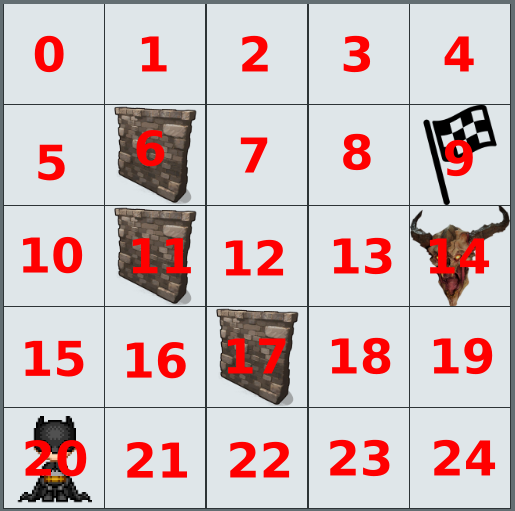
\includegraphics[scale=.4]{img/problemStateEx}}\qquad
    \subcaptionbox{\label{img:problemSolutionEx} Solução}{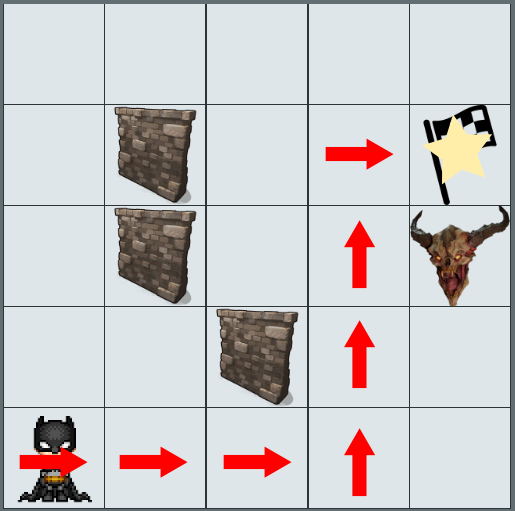
\includegraphics[scale=.4]{img/problemSolutionEx}}
    \vspace{1.5em}
    \legend{\textbf{Fonte:} O Autor}
\label{fig:dag}
\end{figure}

\begin{table}[!htb]
    \centering
    \begin{tabular}{c|c|c|c|c}
            & UP        & DOWN      & LEFT      & RIGHT     \\ \hline
        0   & 2,036     & 3,539     & 2,090     & 5,136     \\
        1   & 3,112     & 2,965     & 4,019     & 6,719     \\
        2   & 4,634     & 4,575     & 4,910     & 9,256     \\
        3   & 7,253     & 13,260    & 6,720     & 13,36     \\
        4   & 11,289    & 20        & 9,250     & 11,322    \\
        5   & 4,147     & 3,144     & 1,406     & 1,004     \\
        6   & 0         & 0         & 0         & 0         \\
        7   & 6,719     & 6,642     & 7,139     & 13,36     \\
        8   & 9,256     & 9,256     & 9,256     & 20        \\
        9   & 0         & 0         & 0         & 0         \\
        10  & 3,548     & 2,898     & 1,090     & 1,130     \\
        11  & 0         & 0         & 0         & 0         \\
        12  & 9,256     & 4,674     & 4,593     &  9,251    \\
        13  & 13,360    & 6,720     & 6,720     & -14,279   \\
        14  & 0         & 0         & 0         & 0         \\
        15  & 3,175     & 3,216     & 0,985     & 3,216     \\
        16  & 1,216     & 3,586     & 2,987     & 1,216     \\
        17  & 0         & 0         & 0         & 0         \\
        18  & 9,256     & 5,153     & 4,720     & 5,153     \\
        19  & -19,999   & 4,076     & 6,720     & 2,966     \\
        20  & 2,988     & 1,216     & 1,216     & 3,586     \\
        21  & 3,216     & 1,586     & 3,216     & 4,185     \\
        22  & 2,185     & 2,185     & 3,586     & 5,153     \\
        23  & 6,720     & 3,153     & 4,185     & 4,185     \\
        24  & 4,956     & 2,184     & 5,153     & 2,183     \\
    \end{tabular}
    \caption{\textit{Q-Table} resultante da execução do experimento.}
    \label{tab:QtableEx}
\end{table}


Estando o personagem inicialmente no estado 20, observando os resultados na \textit{Q-Table}, é
possível traçar o caminho para vitória como o mostrado na Figura \ref{img:problemSolutionEx} que,
notavelmente, é o caminho mais eficiente.
